\documentclass[11pt,a4paper,UTF8]{ctexart}

\usepackage[margin=2.2cm]{geometry}
\usepackage{amsmath}
\usepackage{booktabs}
\usepackage{graphicx}
\usepackage{microtype}
\usepackage[round,authoryear]{natbib}
\usepackage[colorlinks=true,allcolors=blue]{hyperref}

\setlength{\parindent}{2em}
\setlength{\parskip}{0.25em}
\setlength{\emergencystretch}{2em}
\renewcommand{\arraystretch}{1.12}

\title{行为引导不是个性化教育：AI 导师的稳定差异与适应性缺口}
\author{匿名稿中文阅读版}
\date{}

\begin{document}
\maketitle

\begin{abstract}
提示词可以让 AI 导师更多提问、更少揭示答案，或者表现得更加支持学习者。这种变化容易被称为“个性化”，但本文表明，它通常只是较窄的行为引导：模型稳定地向某一教学风格偏移，却不一定适合当前学习者。我们利用大规模教育评测档案中的同题回复，首先检验模型之间是否存在教育行为差异、哪些差异能够跨任务重复，以及共享教学提示如何改变这些差异；随后考察被诱发的行为是否符合人类教师行动、是否反映学习者状态诊断，以及模型能否根据情境选择教学动作。结果显示，模型确实存在少量重复的默认差异。帮助直接性能够跨教学任务迁移，并与独立推断的人类教师行动一致；表达置信度也在四类来源中保持稳定排序。但同一个教学提示会使所有模型明显增加引导、减少直接帮助，同时保留模型特异的剩余差异和响应幅度。这样的引导并不是个性化教育：提示提高了总体教师行动一致率，却在人类教师选择直接讲解时压制了讲解；模型几乎可以完美执行外部指定的提问或讲解动作，试验中的动作选择器却接近随机。多种吸引人的人格解释也没有通过检验。因而，AI 导师评价应当把行为视为“模型--教学指令--学习者情境”的交互结果，并分别检验默认风格、行为引导、动作选择与学习结果。
\end{abstract}

\section{引言}

人们与 AI 导师互动时，很快会注意到不同系统“教得不一样”。面对相同学习者和相同题目，一个模型直接解释，另一个模型继续追问，第三个模型则以更确定的语气作答。因此，在讨论这些差异是否稳定之前，首先需要回答一个更基础的问题：控制题目和生成条件之后，不同模型之间是否仍然存在系统性的教育行为差异？如果存在，这些差异究竟能否跨教学任务重复，还是只反映某一个任务、某一条提示或一般性的生成器指纹？

既有语言模型人格研究往往从人类量表或指定角色开始\citep{jiang-etal-2024-personallm,lee-etal-2025-trait}。这能说明模型可以生成符合某种特质的答案，却不能说明同样的模型排序会在实际教学行为中出现。量表得分还会随措辞和选项顺序变化\citep{shu-etal-2024-dont}；近期研究也质疑，人类心理测量构念对模型是否仍有相同含义\citep{han-etal-2025-personality-illusion,zierahn-etal-2026-arent-human,contreras-2026-native-psychometric}。

教育场景使这些问题既重要又可检验。导师需要决定是讲解还是引导，是揭示答案还是保留学习者工作，一次引入多少信息，以及以多大确定性表达判断。这些行为能够在重复情境中观察，也可以与人类教师行动和学习者状态标签比较。它们还揭示了提示工程中容易忽略的区别：稳定诱发一种教学动作，并不等于为当前学习者选择了正确动作。同一个追问在有价值的错误之后可能合适，在需要直接教学时却可能成为阻碍。

因此，本文提出六个问题：在匹配条件下，不同模型是否具有教育行为差异？哪些差异能够跨教学任务重复，其中是否有差异延伸到教育之外？这些差异能否区别于篇幅、格式和一般作者指纹？共享教学提示能把行为改变多少？不同模型对同一提示的响应是否相同？最后，重复或被诱发的风格能否预测情境适切的教学？本文仅把“教育人格”作为反复出现的可观察行为倾向的简写，并不假定模型具有内在心理状态或与人类等价的特质。

我们正好拥有一个难得的数据条件。EDU Benchmark 档案保存了多个模型在相同题目和共同评测框架下、覆盖教学与通用任务的大量回复。本文先利用这些历史数据筛查候选差异，并控制题目内容和通用作者指纹；再采用配对教学提示、盲评语义测量、人类教师行动、人类金标准学习者诊断，以及一项小规模跨领域亲和性试验做定向验证。这样，新模型调用只用于检验已有数据提出的具体问题，而不是先挑一个量表再制造人格结论。

研究结果形成了一条清楚的主线：模型具有少量重复的默认差异，简洁的教学提示又可以把所有模型稳定推向某一种共同风格；但固定方向的行为偏移并不是个性化教育。先提问提示虽然改善总体行动一致率，却损害需要直接讲解的子集；看似适应性的教学表达没有增加学习者状态信息；几乎完美的动作执行也没有转化为可靠的动作选择。因此，适当的评价对象不是孤立的模型或提示，而是特定模型与教学指令在具体学习者情境中共同形成的行为系统。

\section{相关工作}

行为优先的心理测量包括投射式刺激和与构念匹配的情境\citep{wang-etal-2026-genpt,kocielnik-etal-2026-rethinking}。跨任务研究考察了指定人格在不同诱发格式中的一致性\citep{reusens-etal-2025-persona-consistency}。本文审计的则是：在未指定人格、评测框架一致的情况下，模型作为导师所表现出的默认行为，并依次施加任务、指纹、干预和外部效标控制。我们的定向桥接仅将公有领域的 IPIP 题目\citep{goldberg-etal-2006-ipip}作为一种测量路径，而不把它当作模型行为的真值。

MathDial 定义了教师行动和过早揭示解答\citep{macina-etal-2023-mathdial}；MRBench 与 MathTutorBench 对开放式辅导能力进行了组织\citep{maurya-etal-2025-mrbench,macina-etal-2025-mathtutorbench}。LongTutor 区分历史证据、知识状态诊断和适应性教学\citep{li-etal-2026-longtutor}。Pedagogical Alignment 与 StratL 训练或优化预先定义的脚手架策略\citep{sonkar-etal-2024-pedagogical,puech-etal-2025-steering}；提示调节相较于未调节导师也可能产生负面作用\citep{steindl-etal-2025-prompt}。与本文的情境敏感性问题最接近的是，\citet{borchers-shou-2025-adaptivity}发现模型在学习者情境消融下只表现出有限适应性。导师人格引导\citep{lee-etal-2026-tutor-personas}和基于理论的运行时控制\citep{nkambou-etal-2026-pedrag}关注如何诱发目标策略，PATS 则根据学生人格调整策略\citep{rooein-etal-2026-pats}。本文测量已部署系统中反复出现的默认行为，审计其构念效度，然后再对同一行为实施干预。导师策略预测\citep{ikram-etal-2025-strategy}与反馈失败定位\citep{yasir-etal-2026-feedback}也说明，相比单一的导师总分，更应报告具体行动层面的错误。

“先定策略、再生成回复”并非新概念：既有研究已经联合预测导师策略和回复\citep{wang-etal-2023-strategize}，Tutor CoPilot 则在真实系统中有意保留人类对策略的选择\citep{wang-etal-2025-tutor-copilot}。SLOW 明确区分学习者状态推理与行动选择\citep{wei-etal-2026-slow}。因此，本文的路由测试是对“仅靠提示就能实现模块化”的受控证伪，而不是声称发明了一种两阶段导师。

在教学越狱和学生多轮对抗压力下，答案保留已经得到研究\citep{zhao-etal-2026-shape,zhao-etal-2026-answer-leakage}。真实部署数据也显示，学生普遍会索要答案，而且实际情境可能压过系统原本的设计意图\citep{kobler-etal-2026-students}。因此，我们对学习者行动的分析既不是首次提出答案泄漏或行为引导，也不把策略服从等同于学习收益。

更一般地，IHEval 发现，当不同层级的指令发生冲突时，模型表现会明显下降\citep{zhang-etal-2025-iheval}。因此，学习者的显式请求能否穿透系统层的教学策略条款，本质上是一个指令层级问题，而不是关于同理心、理解学习者或教学适切性的证据。

仅靠身份归因和一个总分仍然不足：词汇特征能够跨领域识别生成模型，而一般“有帮助性”的结论可能随评审器变化而反转\citep{mcgovern-etal-2025-fingerprints,fan-etal-2026-helpfulness}。我们也不假定提示生成的模拟学生能够测量真实学习；近期评测发现其语言、行为和认知保真度都较弱\citep{scarlatos-etal-2026-simulated}。因此，本文把客观诊断与证据检索视为前置能力，把学习增益留给未来的前瞻性研究。

\section{数据与治理}

核心面板包含六个冻结的已部署配置：MiniMax-M3、MiniMax-M2.7、GLM-5.2、DeepSeek-V4-Pro、Doubao-Seed-2.0-Pro 和 Qwen3.5-4B。对于每一道题，我们只保留六个模型都成功生成的回复。六个教学任务分支共得到 31,638 条回复；四个通用负控制任务族共得到 57,516 条回复。包含九个模型的 MathDial 面板另外加入三个配置，共含 26,586 条回复。LongTutor 提供较长的学习者历史，MathTutorBench 则在标准和困难情境下提供通用提示与 LearnLM 风格教学提示的配对数据。

\begin{table*}[t]
  \centering
  \small
  \resizebox{\textwidth}{!}{%
  \begin{tabular}{lrrrl}
    \toprule
    \textbf{面板或效标} & \textbf{模型数} & \textbf{共享单元} & \textbf{回复数} & \textbf{主要作用} \\
    \midrule
    核心教学任务 & 6 & 5,273 题 & 31,638 & 重复教学行为 \\
    通用控制任务 & 6 & 9,586 题 & 57,516 & 作者身份控制 \\
    MathDial 干预 & 9 & 2,954 题--分支 & 26,586 & 引导与离散度 \\
    盲评语义面板 & 6 & 358 情境--分支 & 2,148 & 信度与迁移 \\
    LongTutor 客观任务 & 6 & 1,000 段历史 & 6,000 & 诊断边界 \\
    认识论档案 & 6 & 4 类来源 & -- & 置信表达重复性 \\
    亲和性试验 & 5 & 12 组匹配冲突 & 280 次调用 & 跨领域行为 \\
    人类教师行动 & -- & 18,541 轮 & 18,541 & 分类器训练 \\
    前瞻析因试验 & 5 & 32 道题 & 2,560 & 成分可寻址性 \\
    顺序复现 & 5 & 8 道固定题 & 640 & 顺序稳健性 \\
    \bottomrule
  \end{tabular}}
  \caption{证据来源以及保留依赖结构的分析单元。估计不确定性时，共享单元不会因为模型数量而被重复计数。}
  \label{tab:data}
\end{table*}

MathDial 原始数据提供人类教师的下一步行动（\texttt{probing}、\texttt{focus}、\texttt{telling} 和 \texttt{generic}）。LongTutor 提供人类金标准的知识状态诊断，以及按照参考答案评分的历史证据任务。我们用 SHA-256 固定了 84 对相关的预测文件与汇总文件。由于 84 次运行中只有 22 次保留了温度参数，且全部 84 次运行都缺少随机种子和提示版本信息，因此无法精确重新生成提供方的原始回复。

公开分析产物只保存标识符、哈希、特征、分数和推断标签，不保存原始回复。虽然 LongTutor 论文说明其数据采用 CC BY 4.0 许可，我们仍出于隐私最小化原则不公开纵向学习者历史。只有在获得明确授权后，我们才将外部语义样本发送给评审模型。

\section{方法}

\subsection{透明特征与迁移}

我们以确定性规则统计回复长度、结构、格式、问题、称呼、表扬、鼓励、保留表达、祈使语、历史引用、答案揭示、解释和诊断标记。在完全相同的题目内部，将各模型特征相对于模型均值中心化，再在基准内部标准化。多项逻辑回归在完整留出一个任务族的条件下预测模型身份。相同流程也应用于通用任务，作为负控制：如果通用任务同样具有较强可识别性，就不能把作者指纹重新命名为教学特征。

对配对提示，我们在同一情境、同一模型内，用教学提示分支的特征减去通用提示分支的特征。Bootstrap 重采样以情境为单位，同时保留同一情境中六个相互关联的模型回复。我们既测量每个模型的方向性效应，也测量模型间行为剖面的离散度。

\subsection{质量、行动与学习者状态}

质量预测每次留出一个候选模型。以完全相同题目的固定效应作为基线，再依次加入篇幅特征和策略特征。在两位评审器对字节完全一致回复所给的分数上，我们进行评审器互换检验。另有 482 组专家标注的正负样本对，每一对以两种顺序展示，用于审计三个评审器。

我们用 18,541 轮人类教师对话训练了三个 TF--IDF 线性 SVM 变体，五折划分按数学题目分组。随后比较生成回复所对应的推断行动与人类教师的真实下一步行动。LongTutor 分析则按照完全相同的历史和模型，把教学、诊断与证据任务连接起来。留出模型的预测先纳入完全相同历史的固定效应，再加入教学得分。

\subsection{历史档案中的候选教育行为}

我们从导师必须作出的可观察决策出发选择维度，而不是先套用人类特质标签。候选维度必须同时满足四项要求：能够从开放回复中观察；具有明确的教育含义；能够在异质任务之间比较；并且可以通过跨任务重复或外部效标被证伪。

第一类是\textbf{帮助分配}。帮助直接性测量模型是否揭示答案、步骤或完整解释；引导作答测量模型是否通过问题和提示推进对话；自主支持测量模型是否把实质性的推理或选择留给学习者。三者相关但不是简单反义，一条回复可以先解释再提问，提问本身也不必然保留学习者控制。第二类是\textbf{学习者取向}。情感温暖描述鼓励和积极语气；诊断具体性描述模型是否指出具体证据或误解；个性化描述内容或策略是否根据当前学习者调整。温暖语言不等于准确诊断，准确诊断也不等于后续策略已经适配。第三类是\textbf{教学推进}，包括单轮信息负荷、模型规定教学方向的主动性，以及是否给出可以立即执行的下一步。第四类是\textbf{认识论表达}，包括谨慎措辞、表达置信度、面对新证据的修正，以及证据不足时的拒答；这些指标都不被等同于正确性或校准。

这四类维度分别回答：模型给多少帮助、如何与学习者互动、如何推进教学过程，以及如何表达自身知识状态。只有当模型排序能跨任务来源迁移时，才把某个行为称为重复出现。可靠标注、跨任务重复和独立教育效标是三个不同证据层级。六个模型配置之间的相关只作描述，不作为模型总体的潜变量证据。

\subsection{盲评语义面板与冻结层级}

确定性抽样最初包含 360 个“情境--分支”批次和 2,160 条回复：40 个 LongTutor 情境、80 组标准 MathDial 配对、40 组困难配对，以及 80 个苏格拉底式情境。三位评审器在八个双极 1--5 分维度上编码：帮助直接性、引导作答、学习者自主支持、情感温暖、诊断具体性、个性化、认知负荷和认识论谨慎。模型身份被隐藏，且每位评审器、每个批次中的回复顺序都独立随机化。验证性分数采用三位评审器的中位数。

经过三轮、每轮三次尝试，仍有一条 DeepSeek 标注无法获得。在正式分析之前，且尚未查看受影响分数时，我们删除了该通用批次及其预先指定的教学提示配对批次，并对所有评审器采用同一删除规则。因此，完整案例面板含 358 个批次、2,148 条回复和 1,074 次批次标注，技术性流失率为 0.56\%。

八个维度全部保留并报告。冻结的证据层级要求：（i）ICC(3,k)$\geq .60$、有足够取值范围、逐一留出评审器后的剖面相关 $\rho\geq .70$，且提示效应不出现符号反转；（ii）在控制完全相同情境后仍有非零模型方差，并且跨任务 ICC 或任务相关中位数 $\geq .50$；（iii）至少通过一个独立效标，即质量/行动、提示/行动，或经过 BH 校正的人类金标准诊断关系。这样可以把可靠测量、跨任务重复和外部行为验证分开表述。

\subsection{前瞻性成分干预}

在查看任何生成回复或效应之前，我们冻结了 32 道合成小学数学题，以及一个完整的 $2\times2\times2$ 干预设计，三个因素分别为系统条款中的“先提问”“揭示答案”和“温暖语气”。每个析因单元再与学习者的“直接帮助”或“探索”请求交叉，并在五个可调用模型路由上运行，共 2,560 次调用。确定性检测器分别判断：第一个类似句子的片段是否为问题、是否揭示了正确答案，以及是否出现冻结的鼓励词表。所有析因单元、模型、题目族、次要表层结果，以及二阶和三阶交互作用均完整报告。

一个成分要通过验证，必须超过注册的目标效应阈值（问题和答案为 .60，语气为 .30），在每个模型上的效应都为正，并且目标效应至少是最大主要交叉效应的两倍。学习者请求适应性另设 .10 阈值。由于父试验队列按字典序排列，我们在仍未查看结果时，冻结了一个含八道题的重放试验：提示逐字节相同，顺序由模型特异的 SHA-256 决定，并保证每个连续区块中的 16 个“请求--策略”单元完全平衡。只有当两个面板都通过，且每个模型在匹配的父试验子集和复现中均呈正效应时，才能称为顺序稳健；重放试验只能降低结论等级，不能升级。

在查看汇总效应之后，我们又冻结了一项只能降级的检测器审计。与结果无关的哈希抽样得到 480 条回复（父试验 320 条、重放试验 160 条）。三位盲评者对 48 个、每个包含十条回复的批次进行标注，不知道模型、因素、检测器或效应信息。验证要求多数标注覆盖率 $\geq .95$、平衡准确率 $\geq .90$ 且 Bootstrap 下界 $\geq .80$、Cohen's $\kappa\geq .70$；若失败，则结论只能限于检测器的字面含义。

\subsection{推断、多重比较与冻结时点}

推断单元随研究主张而定（表~\ref{tab:data}）。跨任务归因报告留出任务族的非加权宏平均。提示效应区间以底层情境为单位重采样，同时保留所有与模型联结的行；评审调用先在每条回复上取中位数，绝不将其视为独立教育案例。质量模型报告每一个留出模型折，精确符号检验以折而非回复作为重复。提示检验在每个难度内，对 48 个“模型 $\times$ 维度”对比做 BH 校正；语义诊断则在每种结果内部进行 BH 校正。

多评审方案冻结于 1,080 次标注中的第 311 次；当时所有标注都来自第一位评审器，第二和第三位评审器的结果均不可见。由于单评审器方向已被查看，这属于前瞻性的多评审冻结，而不是完整预注册。论文的决策阈值冻结于 1,080 次标注中的第 637 次，当时第三位评审器和所有 LongTutor 语义标注仍不可见；后续的多重比较修正也先于所有语义 LongTutor 结果。分析器哈希和技术性流失修正均保留在审计记录中。

\subsection{通用人格桥接}

在新增生成之前，我们先以理论为起点审计历史档案，把 Big Five、HEXACO 的诚实--谦逊、Dark Triad、Schwartz 价值观、邻近效度构念、测量路径与稳定性扰动映射到现有任务。候选语言剖面必须能够在教学以外复现、迁移到默认教学行为，并通过篇幅和组织风格控制。档案审计可以选出、但不能确认一个前瞻性后续候选。

审计最终选出“亲和性”。我们冻结了五个模型配置、十二组匹配的教育/非教育冲突、四种条件（默认、无关界面情境、高亲和与低亲和）、十道 IPIP 宜人性题目和十二道强制选择题。三位盲评者在五个维度上评价开放回答。默认稳定性必须同时满足：ICC(3,k)$\geq .70$；跨领域及扰动前后剖面相关 $\rho\geq .70$；扰动导致的绝对均值变化 $\leq .25$；模型间标准差 $\geq .15$。提示可引导性，以及自我报告/强制选择与开放行为的收敛，是彼此分离的冻结主张。

\section{结果}

\begin{figure*}[t]
  \centering
  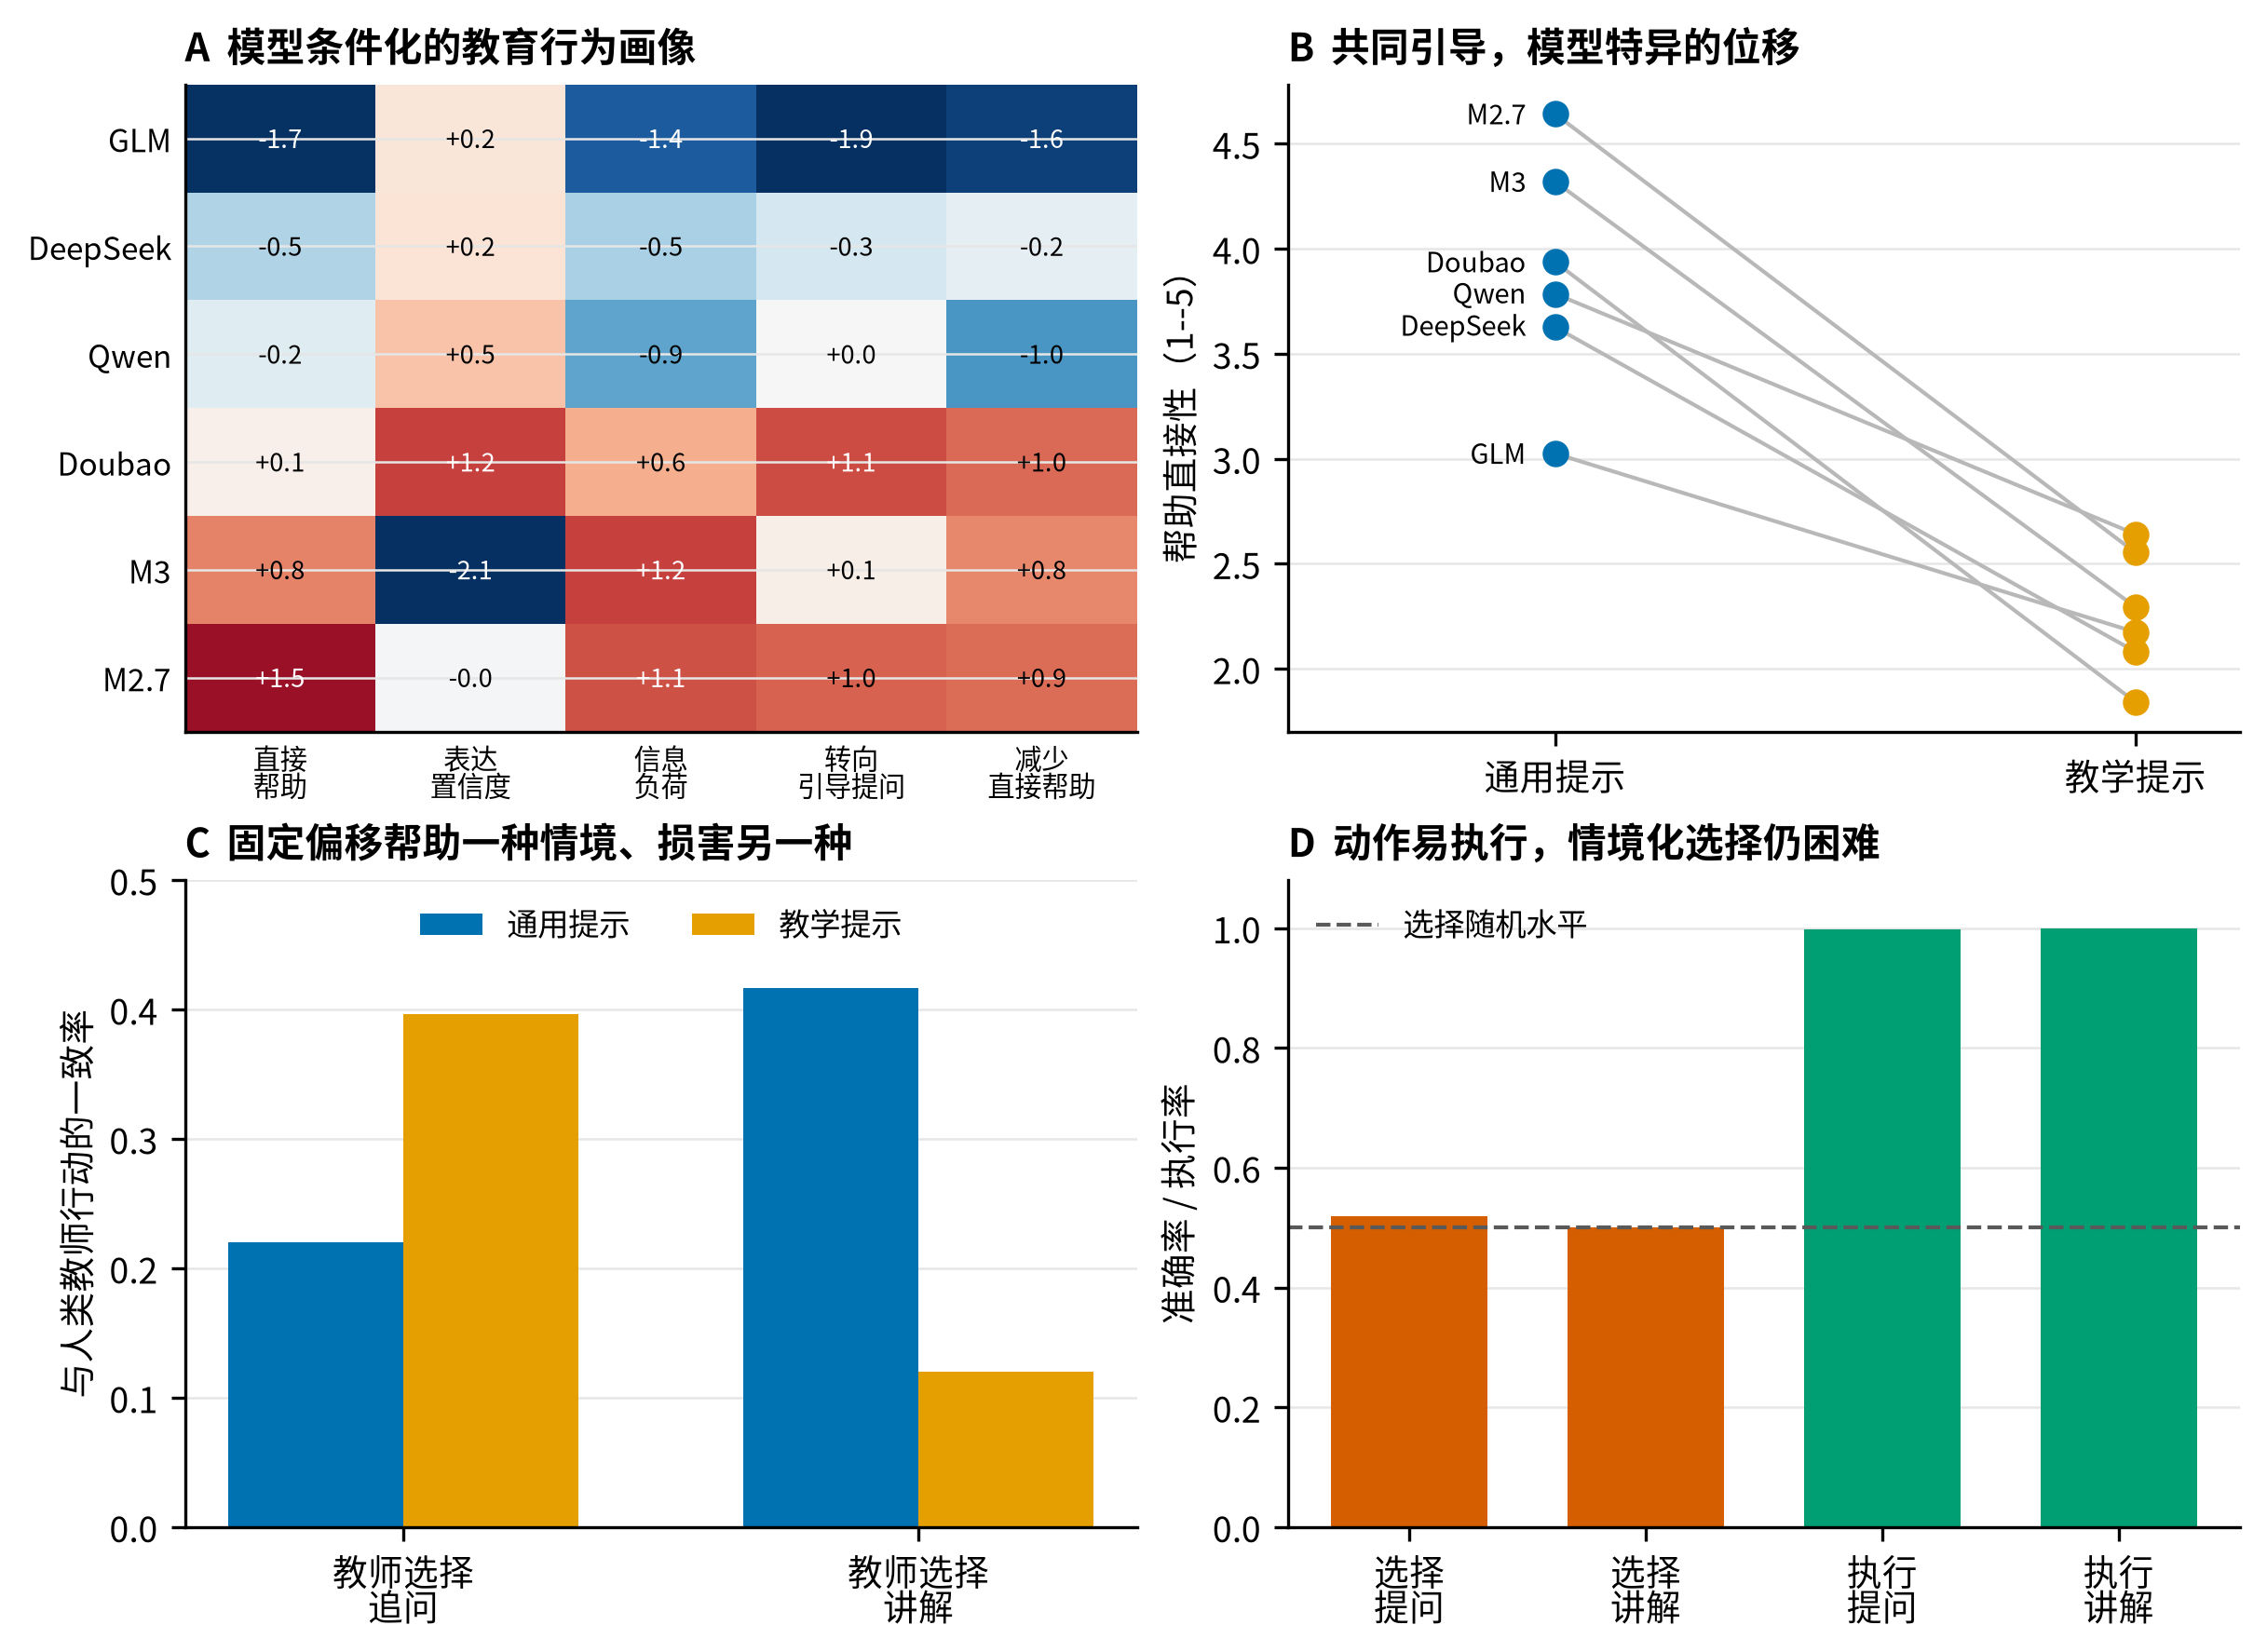
\includegraphics[width=\textwidth]{../figures/main_findings_zh.png}
  \caption{行为引导能够改变教学风格，却不自动产生个性化。（A）六个冻结模型配置具有不同的五轴行为画像；各列在当前面板内标准化，只描述相对行为，不是能力分。（B）共享教学提示使所有模型减少直接帮助，但移动幅度不同。（C）固定偏移提高了追问情境的一致率，却损害直接讲解情境。（D）模型能够执行指定动作，试验中的选择器却不能可靠地根据情境选择动作。}
  \label{fig:main}
\end{figure*}

\subsection{模型之间存在差异，但只有少数差异能够重复}

最清楚的教育差异，是模型多愿意直接提供帮助。帮助直接性的盲评信度较高（ICC(3,k)=.905），能够跨教学任务复现（跨任务 ICC=.629；任务相关中位数 $\rho=.647$），并与独立行为效标一致：被分类为人类式 \texttt{telling} 的回答，比 \texttt{probing}/\texttt{focus} 高 1.360 分。默认模型均值相差约 1.65 分，从最不直接的 GLM 到最直接的 MiniMax-M2.7。这是历史档案中最有力的重复教育行为证据（图~\ref{fig:main}A）。

表达置信度构成第二种较窄但清楚的差异。在四类独立来源中，其模型剖面具有较高稳定性（ICC(3,1)=.852；任务相关中位数 $\rho=.886$）：Doubao 最高（.977），MiniMax-M3 最低（.878）。这里测量的是回答表达得多么确定，而不是回答是否正确。它也不能替代修正或拒答倾向：Qwen 的表达置信度很高（.956），同时在不可回答题上的拒答率也是最高的（.912）。

表~\ref{tab:model-profiles} 把证据较强的结果转化为模型层面的相对评价。帮助直接性是控制完全相同题目后的中心化默认分数；提示变化是在标准和困难情境中、1--5 分语义量尺上的平均变化。更加直接、更加确定或更容易被提示改变，都不等于教学质量更高。

\begin{table*}[t]
  \centering
  \small
  \resizebox{\textwidth}{!}{%
  \begin{tabular}{lrrrl}
    \toprule
    \textbf{冻结配置} & \textbf{默认直接性} & \textbf{表达置信度} & \textbf{提示后直接性变化} & \textbf{证据范围内的行为评价} \\
    \midrule
    MiniMax-M2.7 & .803 & .941 & $-2.089$ & 默认最直接；教学提示下变化很大 \\
    MiniMax-M3 & .408 & .878 & $-2.026$ & 默认较直接；表达置信度最低；变化很大 \\
    Doubao-Seed-2.0-Pro & .071 & .977 & $-2.096$ & 默认接近面板均值；表达置信度最高；变化很大 \\
    Qwen3.5-4B & $-.113$ & .956 & $-1.144$ & 默认略少直接帮助；表达置信度高；变化较小 \\
    DeepSeek-V4-Pro & $-.324$ & .948 & $-1.546$ & 默认较少直接帮助；提示变化居中 \\
    GLM-5.2 & $-.845$ & .948 & $-.851$ & 默认最少直接帮助；额外提示变化最小 \\
    \bottomrule
  \end{tabular}}
  \caption{核心六模型面板的行为画像。数值仅描述冻结部署配置在所抽取任务和提示条件下的相对行为，不是模型家族属性，也不是教学质量排名。}
  \label{tab:model-profiles}
\end{table*}

另一些维度能可靠测量，却不能支持同样强的解释。认知负荷可以跨任务复现（ICC=.663；中位数 $\rho=.677$）；引导作答虽然评分可靠，但跨任务稳定性较弱（ICC=.475；中位数 $\rho=.468$）。表~\ref{tab:semantic-decisions} 保留全部预设维度，包括没有通过的维度。

\begin{table*}[t]
  \centering
  \small
  \resizebox{\textwidth}{!}{%
  \begin{tabular}{lrrrrl}
    \toprule
    \textbf{维度} & \textbf{ICC(3,k)} & \textbf{任务 ICC} & \textbf{任务 $\rho$ 中位数} & \textbf{反转数} & \textbf{最高保留层级} \\
    \midrule
    帮助直接性 & .905 & .629 & .647 & 0 & 重复行为且通过独立效标 \\
    引导作答 & .963 & .475 & .468 & 0 & 仅可靠测量 \\
    学习者自主支持 & .819 & .610 & .734 & 1 & 无 \\
    情感温暖 & .937 & .479 & .714 & 3 & 无 \\
    诊断具体性 & .924 & .203 & .371 & 1 & 无 \\
    个性化 & .832 & .340 & .257 & 1 & 无 \\
    认知负荷 & .855 & .663 & .677 & 0 & 重复行为 \\
    认识论谨慎 & .580 & .035 & .129 & 0 & 无 \\
    \bottomrule
  \end{tabular}}
  \caption{全部预先指定的语义维度都保留并展示。可靠测量、跨任务重复与外部行为验证是不同层次的证据。}
  \label{tab:semantic-decisions}
\end{table*}

这些语义差异不能简化为篇幅：在留出教学任务上，语义维度识别模型的准确率为 .322，篇幅为 .239，随机水平为 .167。但通用任务反而更容易识别模型（组合透明特征 .372，教学策略特征 .242），跨领域结构也没有保持（Mantel $r=.296$，$p=.307$）。因此，能够认出模型只是必要的负控制，不足以证明教育人格。

\subsection{共享提示造成共同偏移，却没有生成共同导师}

同一个显式教学提示带来很大且方向一致的共同变化。九个模型在标准和困难情境中都提出更多问题、生成更短回复；模型间离散度降为通用提示基线的 .763（95\% CI [.738, .794]）。盲评中，帮助直接性分别下降 1.709 和 1.542 分，引导作答上升 2.470 和 2.171 分，认知负荷下降 .759 和 .721 分。帮助直接性的提示位移，与默认模型之间的整个差距大致相当。这证明简洁指令可以有效改变行为分布，但所有学习者情境都被推向同一方向，因此它本身不是个性化。

但共同变化没有让模型变得完全相同。跨提示的模型识别率仍为 .301 和 .297，都高于 .167 的随机水平。控制可移动空间后，各模型对提示的响应幅度仍不同，一些模型对的相对排序还会在提示后反转。因此，数据既不支持“人格固定不变”，也不支持“完全由提示词决定”：模型有可区分的默认行为，共同提示会移动所有模型，而移动幅度和提示后的剩余差异具有模型特异性。教学提示不能被当作与底层模型无关、可无损移植的控制层。

\subsection{多种直观人格解释没有通过检验}

最有说明力的反例是“下一步行动可执行性”。教学提示在标准和困难情境中分别使其提高 1.047 和 .880 分，而且所有模型方向一致，说明它很容易被引导。但其跨任务 ICC 为 $-.111$，任务相关中位数为 $-.771$：模型排序不是重复，而是反转。容易被提示改变，不能证明它是稳定默认人格。

关系共同感的测量信度很高（ICC=.945），但它与表层温暖的相关为 .805，并且在苏格拉底面板中没有模型方差。教学主动性因冻结试验信度只有 .657、未达到 .70 而仍属探索性。个性化和诊断具体性也没有跨任务复现，学习者请求则不能可靠改变其所要求的问题或答案行为。温暖或看似适应性的语言，不足以证明模型会根据学习者作出反应。

把通用人类特质直接搬过来也没有得到支持。组织风格在教学以外能够复现（中位数 $\rho=.771$），却与 IFEval 准确率负相关（$\rho=-.886$，精确 $p=.035$），所以不能把它解释为尽责性。谨慎措辞不能证明诚实--谦逊；候选的规范宽容度在两项任务间反向相关（$\rho=-.486$）。这不证明模型完全没有这些特质，只说明现有档案无法识别它们。

\subsection{引导一种风格，不等于提供个性化教育}

把所有模型推向提问，确实会提高与人类教师行动的总体一致率：54 个“分类器--难度--模型”对比全部提高，标准情境为 .091--.114，困难情境为 .145--.180。但困难情境几乎都以追问为目标。对于 48 个真人教师选择 \texttt{telling} 的标准情境，通用提示下的一致率为 .394--.442，教学提示下却降到 .111--.125；直接讲解比例下降 .234--.280。一个稳定、易识别的“苏格拉底式”风格，完全可能在具体情境中稳定地做错选择（图~\ref{fig:main}C）。提示改变的是导师倾向于做什么，并没有推断这个学习者现在需要什么；平均改善与情境适配是两个不同主张。

学习者状态分析显示了第二重分离。在 6,000 个“模型--历史”观测中，教学质量与诊断只有较弱关系（模型内平均 Spearman=.173），与证据准确率几乎无关（$-.010$）。控制完全相同的历史后，仅用题目效应的诊断 AUC 为 .822；加入四个教学维度为 .816，加入维度均值为 .817。听起来适应性的教学，没有补上学习者状态诊断能力。

前瞻析因试验解释了部分原因。显式系统条款能够强力控制先提问和答案揭示，并在不同调用顺序下复现（表~\ref{tab:factorial}）。但学习者提出“直接帮助”或“探索”请求，对答案揭示的影响在父试验和复现中只有 .073 和 .066，低于冻结的 .10 门槛；对先提问的影响很小且方向相反。模型遵循系统层教学指令的能力，远强于根据学习者表达的需要进行调整。

\paragraph{系统条款的控制效果。}

三个操作性终点都通过了父试验的全部注册门槛，并通过了只能降级的顺序复现（表~\ref{tab:factorial}）。在完整面板、匹配的父试验子集和复现中，五个模型的效应全部为正。按题目族计算，父试验中的先提问效应为 .750--.787，复现中为 .750--.863；答案效应分别为 .878--.928 和 .887--.975；鼓励词标记效应分别为 .525--.659 和 .487--.600。因此，汇总效应不是由某一个模型或某一个题目族单独造成的。

\begin{table*}[t]
  \centering
  \scriptsize
  \resizebox{\textwidth}{!}{%
  \begin{tabular}{lrrcrrc}
    \toprule
    & \multicolumn{3}{c}{\textbf{父试验（2,560）}} & \multicolumn{3}{c}{\textbf{复现（640）}} \\
    \textbf{条款} & \textbf{效应 [95\% CI]} & \textbf{选择性} & \textbf{所有模型为正} & \textbf{效应 [95\% CI]} & \textbf{选择性} & \textbf{稳健} \\
    \midrule
    先提问 & .773 [.756, .790] & 10.20 & 是 & .809 [.772, .841] & 12.95 & 是 \\
    揭示答案 & .895 [.883, .908] & 11.35 & 是 & .922 [.900, .950] & 9.52 & 是 \\
    鼓励词表 & .595 [.563, .623] & 5.04 & 是 & .550 [.497, .597] & 5.33 & 是 \\
    \bottomrule
  \end{tabular}}
  \caption{前瞻冻结的成分效应。“选择性”是目标效应除以最大主要交叉效应的绝对值；注册阈值为 2.0。最后一列还要求每个模型在匹配的父试验子集和独立排序的复现中都呈正效应。}
  \label{tab:factorial}
\end{table*}

盲评检测器审计中，先提问检测器的平衡准确率为 1.000（95\% CI [1.000, 1.000]，$\kappa=1.000$），正确答案揭示检测器为 .996 [.989, 1.000]（$\kappa=.992$），二者均通过验证。鼓励词表仅达到 .818 [.787, .847]，$\kappa=.631$，未通过两个冻结门槛。因此，它只能支持“出现字面鼓励标记”，不能支持“语义上的温暖或支持”；这项结果后审计不能升级任何主张。

学习者请求没有表现出相应稳健性。直接帮助请求相对于探索请求，只使正确答案揭示在父试验中增加 .073 [.061, .085]、在复现中增加 .066 [.041, .087]，均低于注册的 .10 门槛。探索请求相对于直接请求，使先提问在两个面板中分别变化 $-.030$ [$-.047$, $-.014$] 和 $-.016$ [$-.037$, .006]。这反映的是指令层级行为，而不是可靠的学习者理解。

可寻址性也不意味着成分独立。温暖语气条款使先提问在父试验中降低 .118、复现中降低 .103。问题$\times$语气对先提问的交互作用分别为 $-.236$ [$-.266$, $-.208$] 和 $-.206$ [$-.256$, $-.162$]；问题$\times$答案$\times$语气的三阶交互则分别为 .203 [.138, .278] 和 .237 [.125, .350]。这些预先指定的交互在复现中保持方向一致，因此结论只能是：这些是可控制的黑箱行为成分，而不是相互正交的潜在人格特质。

在外部指定 ASK 或 EXPLAIN 后，模型分别以 .998 和 1.000 的比例实现行动；两个行动选择器的准确率却只有 .519 和 .500，将选择与执行串联后还低于单次直接生成（$-.058$ 和 $-.077$）。稳定教育风格描述的是模型倾向于做什么，并不能说明它知道何时应该这样做。

\subsection{亲和性得到有限的跨领域支持}

在 22 个历史构念或效度目标中，九个只有部分候选指标，十三个无法识别，没有一个得到验证。组织风格在教学以外的重复性最强（相关中位数 $\rho=.771$），但它与 IFEval 准确率呈负相关（$\rho=-.886$，精确 $p=.035$），从而证伪了“尽责性”解释。只有亲和性被选中：共同体式表达能够迁移到默认教学行为（$\rho=.829$），也能迁移到独立评审的关系联结（$\rho=.771$），尽管它在不同任务间的重复性较弱。

定向试验通过了固定模型面板中的全部重复性门槛。开放回答信度为 ICC(3,k)=.931；五模型剖面能够跨领域迁移（$\rho=.900$，精确 $p=.091$），在一次无关扰动后仍保持一定稳定性（$\rho=.718$，$p=.174$；均值位移 $-.050$），模型间标准差为 .445。高亲和提示减去低亲和提示的平均位移为 1.689 分，五个模型全部为正，但范围从 .444 到 2.917；高亲和提示把模型间标准差压缩到 .201，低亲和提示则把它扩大到 .879。

通用特质的收敛效度未通过。默认 IPIP 自我报告集中在 4.2--4.9，与开放行为的相关为 $-.200$；默认条件下，强制选择全部选择亲和选项。开放回答中的亲和性与表层温暖的相关为 .900。因此，我们可以说这五个模型在所抽取的冲突情境中表现出跨领域的亲和行为差异，而且提示会强烈改变这种行为；不能说该试验验证了 Big Five 宜人性或一般性的人类式人格。

\subsection{主要发现通过了测量检查}

逐一留出评审器后的剖面相关为 .959--.962；模型族残差和候选位置极差均低于注册警戒线。在 14,770 条完全相同回复上，两位质量评审器的 Spearman 相关为 .806，二次加权 $\kappa=.810$；在 482 组专家标注样本对上，单个评审器的一致率为 .817--.844，因此我们不把任何评审器当作人类真值。语义特征使质量 AUC 平均提高 .015，但其中一个留出模型折为 $-.004$。这一结果再次说明，重复出现的风格与教学质量不是同一个对象。

\section{讨论}

\paragraph{重复行为仍然具有条件性。}
帮助直接性和表达置信度能够跨任务重复，多数看似合理的维度不能；即使是能够重复的差异，也会被共享教学提示大幅移动。提示后的剩余模型身份、响应幅度差异和排序反转说明，单独的默认分或提示效应都不能完整描述导师。真正重复的是模型在特定任务与指令条件下表现出的行为倾向。这种条件性本身就具有教育含义：稳定地偏向讲解或追问，只说明模型如何分配帮助，并不说明这种分配适合某个具体学习者。一般作者指纹同样可以重复，却不一定迁移相应教育构念，因此模型可识别性本身不足以证明教育人格。

\paragraph{固定偏移不能替代情境适应。}
教学提示能够可靠改变模型如何行动，却不能证明被诱发的行动是适当的。平均一致率的改善主要来自追问情境；在人类教师选择讲解时，一致率反而显著下降。教学表达没有增加学习者状态信息，接近完美的动作执行也与接近随机的动作选择并存。因此，更准确的结论不是笼统地说提示词“没有效果”，而是：提示词擅长移动行为分布，个性化教育则需要关于学习者的证据，以及在多个教学动作之间作出依赖情境的选择。真实学习结果还是尚未检验的更高一层要求。

\paragraph{完整导师系统才是适当的评价单元。}
本文操纵的是固定生成框架中的提示词和系统层条款，而不是完整 Harness。记忆、检索、学习者建模、动作路由、工具或生成后检查，都可能弥补固定提示的不足。但当前结果不支持把底层模型当作行为中性、彼此可互换的执行器：相同指令在不同模型上产生不同位移，因此即使外围逻辑保持不变，更换模型也可能改变最终导师。端到端评价应当把目标模型与具体教学配置放在一起，报告重复默认、诱发变化、模型特异响应、动作选择准确率和具体情境结果。构念评价也需要同样的约束：行动可执行性容易诱发却不稳定，关系共同感主要重述温暖，组织性不能验证尽责性，自我报告宜人性也不预测开放行为。一致性、可引导性、适应性和教学效果仍然是不同目标。

\section{可复现性与发布}

发布包包含分析代码、冻结的派生表、图、排除规则、前瞻协议和 SHA-256 清单，但不包含原始回复或学习者历史。析因试验与亲和性试验只保留哈希、条件、派生评分和统计量，不保留模型提供方返回的文本。一个命令可以重跑依赖私有输入的语义最终流程，并在覆盖率、主张、隐私结构、图、语法或测试任一环节失败时阻断发布。另一次独立的全新检出验证了全部冻结公开路径及其哈希。GitHub CI 在新的 Ubuntu 运行器上配置 Python 3.13，安装锁定版本的依赖，并重复执行测试、注册主张审计、隐私审计、图重建和干净工作区检查。这些步骤验证的是公开发布包，不能重新创建私有输入或模型提供方回复。匿名英文稿还固定并校验了官方 ACL 样式的哈希，能够生成字节稳定的 PDF。

\section{结论}

在这一有限模型面板中，AI 导师确实存在教育行为差异，其中只有少数能够跨任务重复。共享提示可以强烈引导所有模型，却不会使模型彼此等价。本文最重要的边界来自教育：把导师推向提问、保留答案或温暖表达，并不会自动产生个性化教育。同一个固定偏移可以帮助追问情境、损害讲解情境；模型即使几乎完美地执行指定动作，仍可能无法从学习者情境中选择它。因而，AI 导师评价应当面向“模型--教学指令--学习者情境”组成的系统，并把行为重复、提示引导、动作选择和学习结果分开检验。

\section*{局限性}

核心面板只有六个系统；回复数量不会创造新的模型重复，因此本文不作模型总体或模型家族层面的推断。大多数质量结果由 LLM 评审，但我们加入了评审器互换、专家样本对校准、人类行动标签和人类金标准诊断作为检查。与人类行动一致不等于产生学习收益；真实教学效能需要在前瞻性学习者中使用客观的前测/后测进行检验。

亲和性试验只有五个模型配置、十二组合成冲突和一次无关扰动。精确剖面检验功效不足，生成模型与评审模型的家族有所重叠，主要评分也不能与表层温暖区分。只有在加入更广泛的扰动、行为博弈和更大的独立模型面板之后，才可能提出通用人格主张。

前瞻析因试验采用合成的小学数学情境和表层检测器。结果后盲评审计验证了先提问和正确答案揭示，但鼓励词表未通过语义温暖验证，因此只能按字面报告。五个终点都是特定时点的提供方快照，八道题的重放试验发生得更晚；提供方版本漂移和重复提示缓存无法与请求顺序稳健性完全分离。成分效应不是学习结果，复现出的交互也排除了把这些条款当作独立潜在特质的解释。

模型提供方的系统提示、别名更新和服务后端均不可控。由于大部分运行设置、全部随机种子和全部提示版本没有保留，生成结果无法精确复现。结论适用于冻结的已部署配置，而不是不可变的模型权重。语义完整案例规则是在提供方失败之后、正式分析之前冻结的；0.56\% 的配对技术性流失已完整报告。

\section*{伦理声明}

本研究分析已有的模型回复和教育历史。公开产物使用哈希和派生测量，不包含原始学习者历史或原始回复。外部语义标注只使用获得明确授权的终点和冻结载荷。模型条件下的差异不应被解读为人类特质、人口统计属性，也不能作为某个系统改善学习的证据。部署时应检验真实学习者结果并保留教师监督，尤其需要警惕统一的苏格拉底式策略可能扣留学习者实际需要的直接帮助。

\bibliographystyle{plainnat}
\bibliography{../references}

\end{document}
